\title{2. Lineární a mocninné funkce}
\author{Jakub Sláma}
\date{25.4.2025}

\maketitle

\section{Lineární a mocninné funkce}

\subsection{Lineární funkce}
\textbf{Definice funkce:} Množina sdružených číselných dvojic, pro které platí, že hodnota každého jednoho $x$ z definičního oboru náleží právě jedno $y$ z oboru hodnot. \\ \\ 
Předpis funkce: $f: y=f(x)$ \\
Grafem funkce $f$ je množina všech bodů roviny, které mají souřadnice $[x;f(x)]$  \\ \\
\textbf{lineární funkce:}
Grafem lineární funkce je přímka. $D(f) \in R$. 
Lineární funkcí rozumíme takovou, která má předpis:
$$
    f:y=kx+q
$$
$$
    k,q \in \mathbb{R}  
$$
kde $k$ je směrnice, jejíž hodnota udává strmost stoupání/klesání přímky a $q$ udává průsečík přímky s osami x a y. A pro hodnoty k platí: \\


\begin{tabularx}{0.8\textwidth} { 
  | >{\raggedright\arraybackslash}X 
  | >{\centering\arraybackslash}X 
  | >{\raggedleft\arraybackslash}X | }
 \hline
  k & co se děje s funkcí & viz.\\
 \hline
 $k>0$      &   funkce je rostoucí  & Figure 2\\
 $k=0$      &   konstantní         & Figure 3\\
 $k<0$      &   klesající          & Figure 4\\
\hline
\end{tabularx}


\begin{figure}[H]
        \centering
        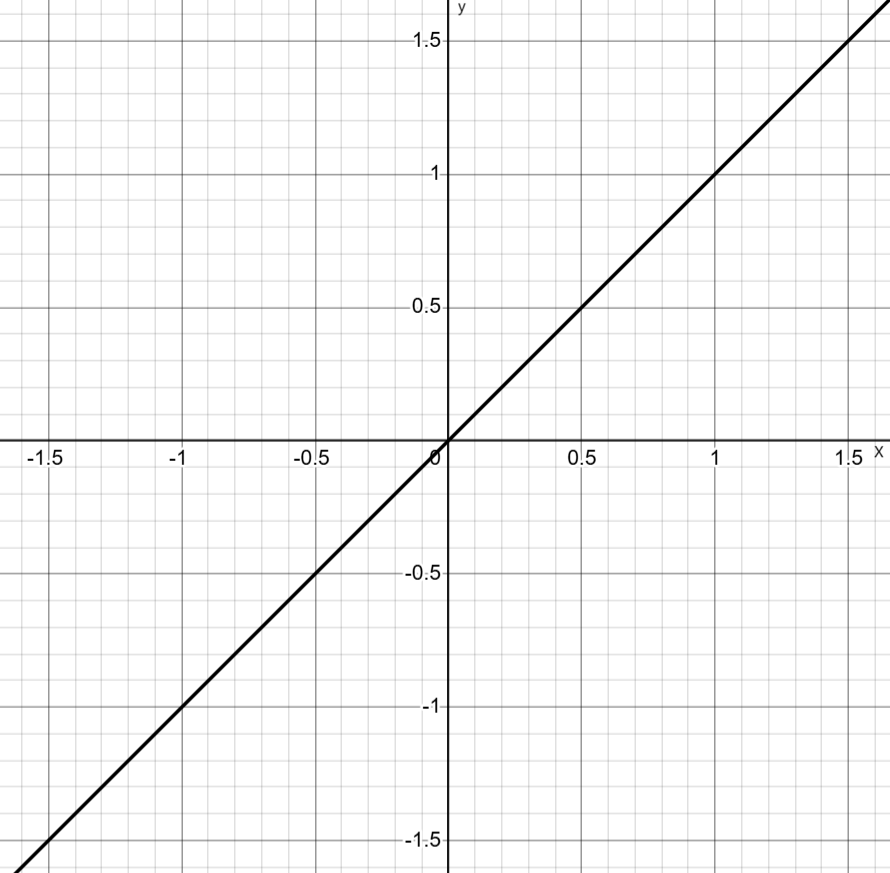
\includegraphics[width=0.4\linewidth]{img/2_graf_y=x.png}
        \caption{$f(x):$ $y=x$}
        \label{fig:enter-label}
    \end{figure}

\begin{figure}[H]
        \centering
        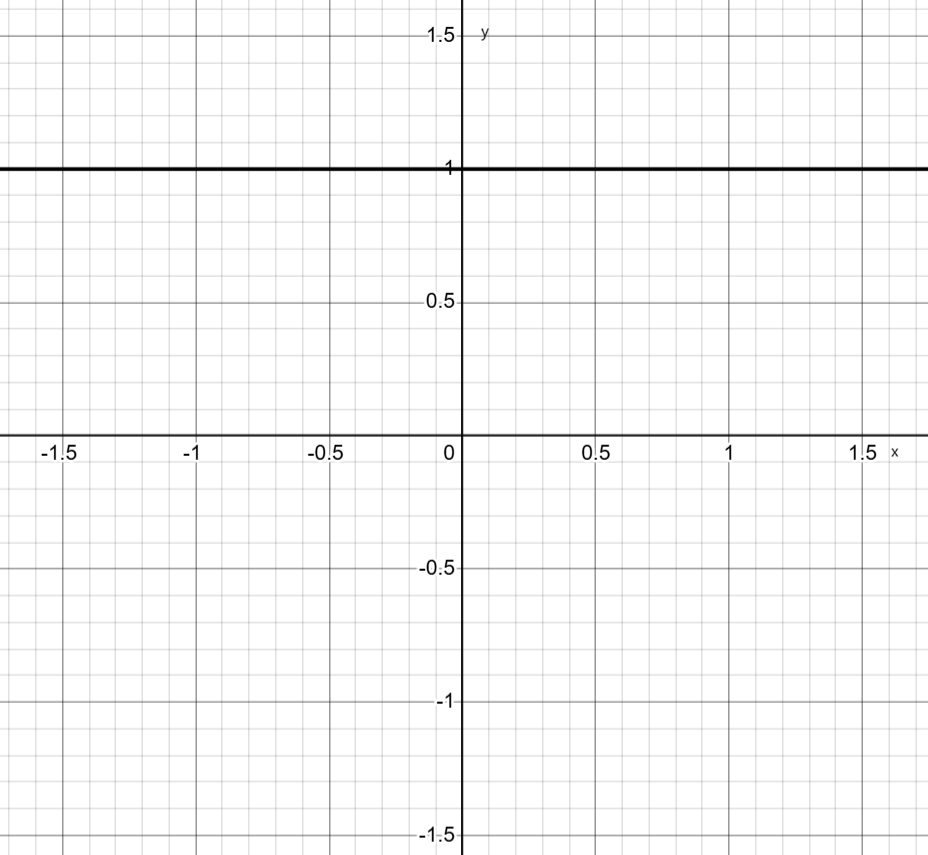
\includegraphics[width=0.4\linewidth]{img/2_graf_y=0x+1.png}
        \caption{$f(x):$ $y=0x+1$}
        \label{fig:enter-label}
    \end{figure}

\begin{figure}[H]
        \centering
        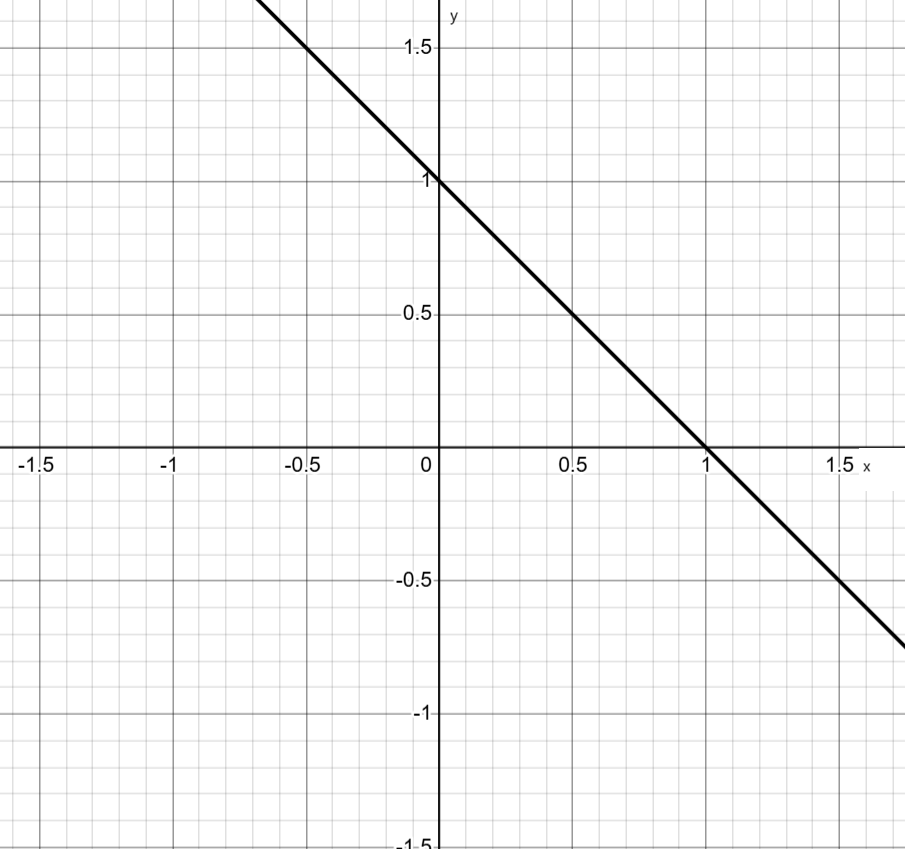
\includegraphics[width=0.4\linewidth]{img/2_graf_y=-x+1.png}
        \caption{$f(x):$ $y=-x+1$}
        \label{fig:enter-label}
    \end{figure}

\subsection{Mocninná funkce pro $n \in \mathbb{N}$ (celá čísla)}
Mocninná funkce má předpis: $y=x^n$, kde $n \in \mathbb{N}$. Vlastnosti se liší pro sudá a lichá $n$
Pro předpis$y=x^n$, kde $n \in \mathbb{N}$ a platí: \\

\begin{tabularx}{0.8\textwidth} { 
  | >{\centering\arraybackslash}X 
  | >{\centering\arraybackslash}X 
  | >{\raggedleft\arraybackslash}X | }
 \hline
  \textbf{sudá funkce} & \textbf{lichá funkce}\\
 \hline
 $n$ je sudé      &   $n$ je liché  \\
 \hline
 $D(f)=\mathbb{R}$      &   $D(f) = \mathbb{R}$         \\
 \hline
 $H(f)=\langle0;\infty)$      &   $H(f) = \mathbb{R}$         \\
 \hline
 je sudá      &   je lichá          \\
 \hline
 Je omezená z dola, shora omezená není      &   není shora ani zdola omezená          \\
 \hline
 není prostá *     &   je prostá          \\
 \hline
 klesající na $(-\infty;0\rangle$ a rostoucí na $\langle0;\infty)$      &      je rostoucí v $\mathbb{R}$       \\
 \hline
 má v bodě 0 minimum $f(0) = 0$      &           nemá maximum, ani minimum  \\
\hline
nemá maximum $f(0) = 0$      &             \\
\hline
viz. Figure 5     &    viz. Figure 6         \\
\hline
\end{tabularx} \\ \\
 *(Prostá funkce je v funkce, která žádnou funkční hodnotu nenabývá vícekrát)

\begin{figure}[H]
        \centering
        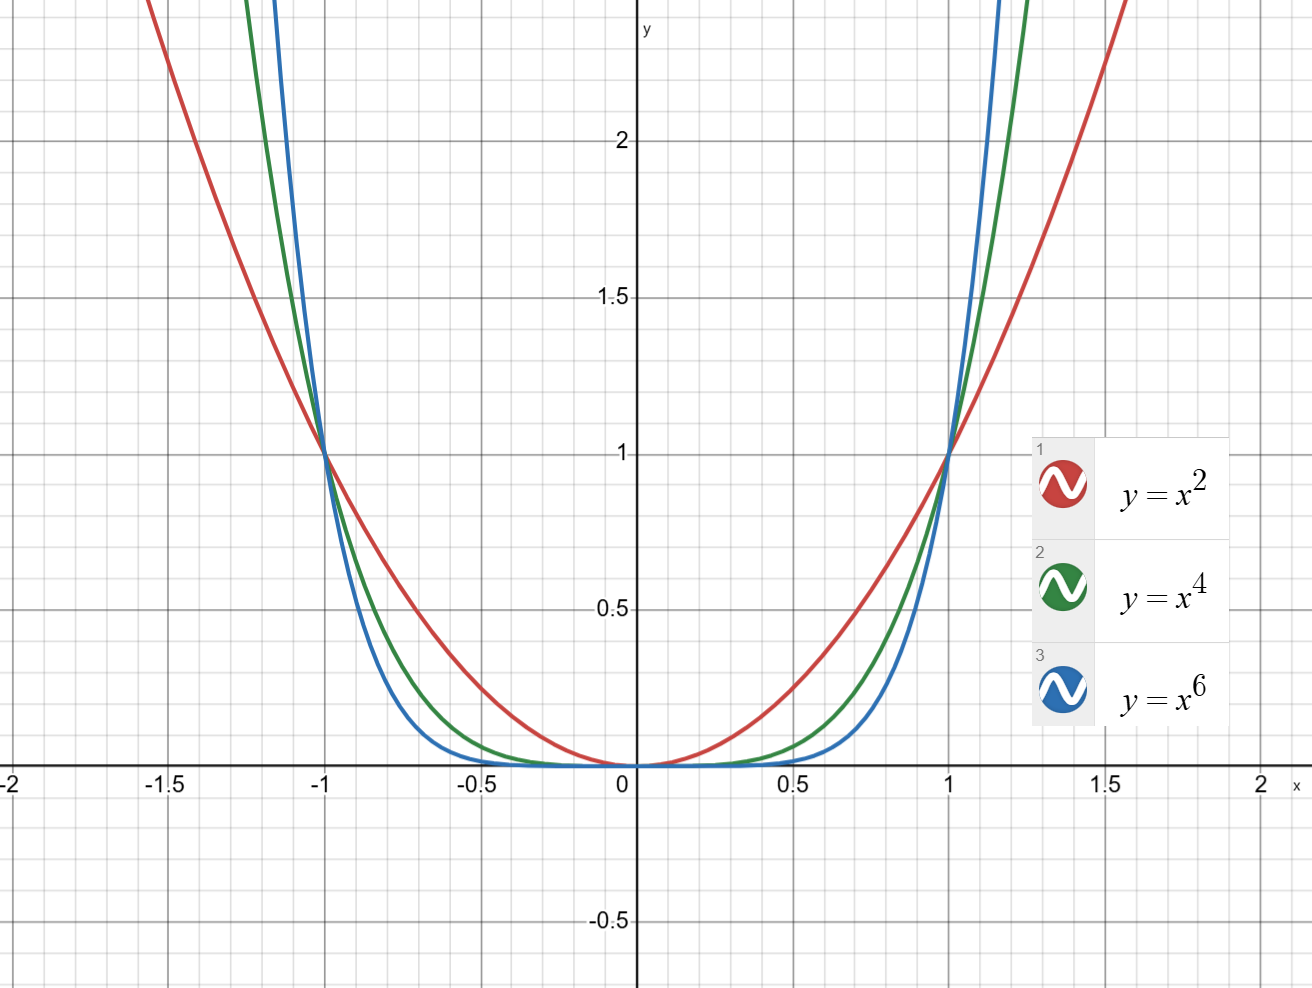
\includegraphics[width=0.5\linewidth]{img/2_sude_fkce.png}
        \caption{grafy funkcí s sudými mocninami} 
        \label{fig:enter-label}
    \end{figure}

\begin{figure}[H]
        \centering
        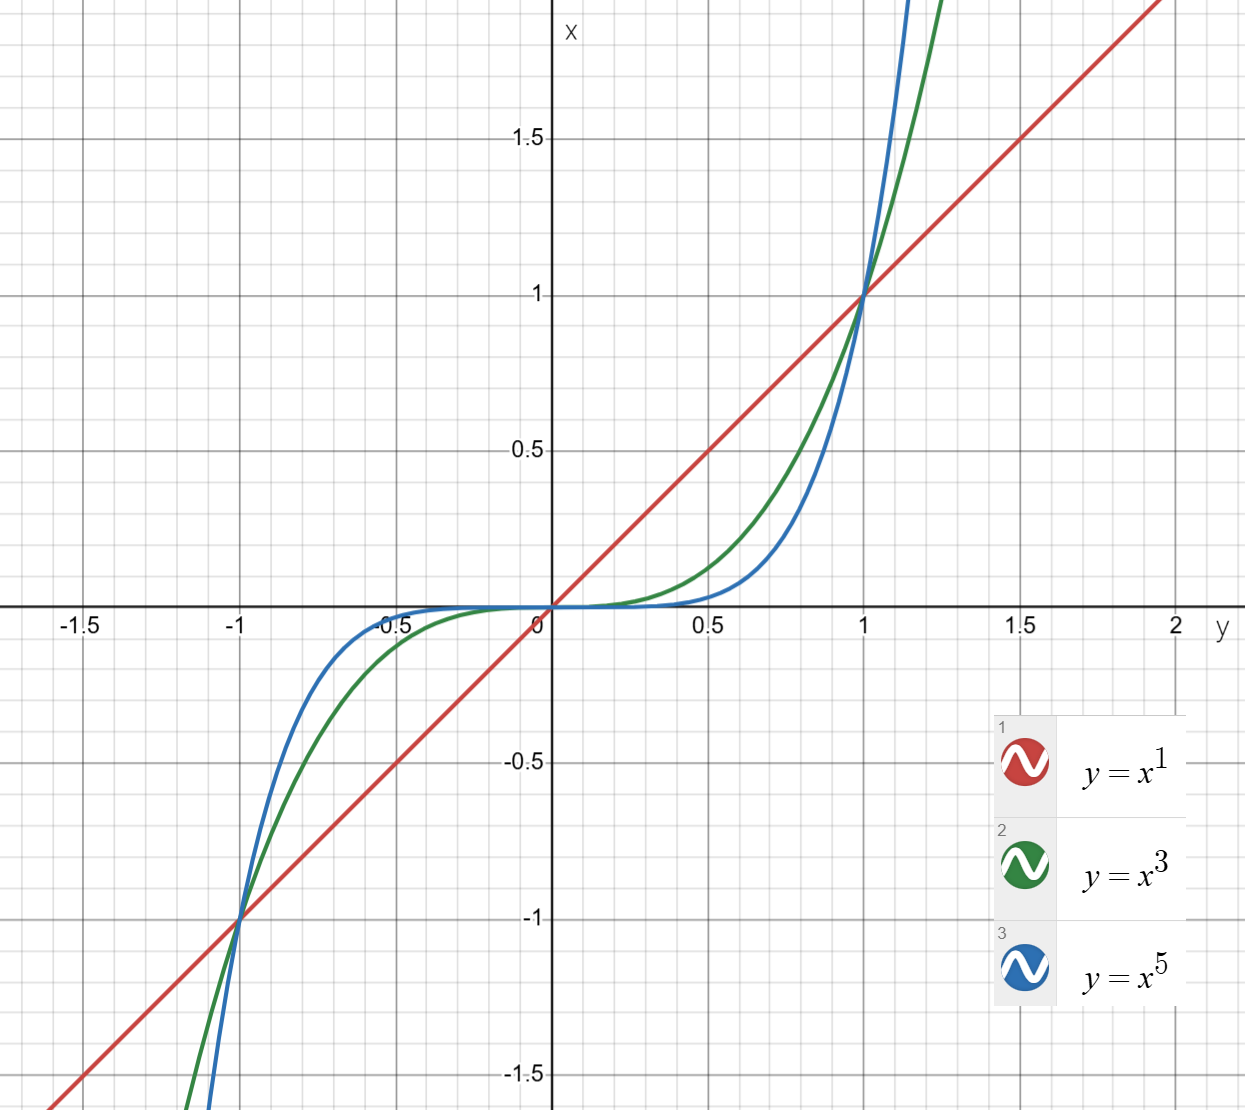
\includegraphics[width=0.5\linewidth]{img/2_liche_fkce.png}
        \caption{grafy funkcí s lichými mocninami}
        \label{fig:enter-label}
    \end{figure}

\subsection{Lineární lomená funkce}
lineární lomená funkce je každá funkce daná předpisem 

$$
f: y=\frac{ax + b}{cx+d}
$$
kde: \\ $a,b,c,d \in \mathbb{R} \\ c \neq 0 \\ ad \neq bc$
Tato funkce je vždy prostá na celém $D(f)$. Grafem je hyperbola s středem v bodě $[-\frac{d}{c}; \frac{a}{c}]$.
\begin{figure}[H]
        \centering
        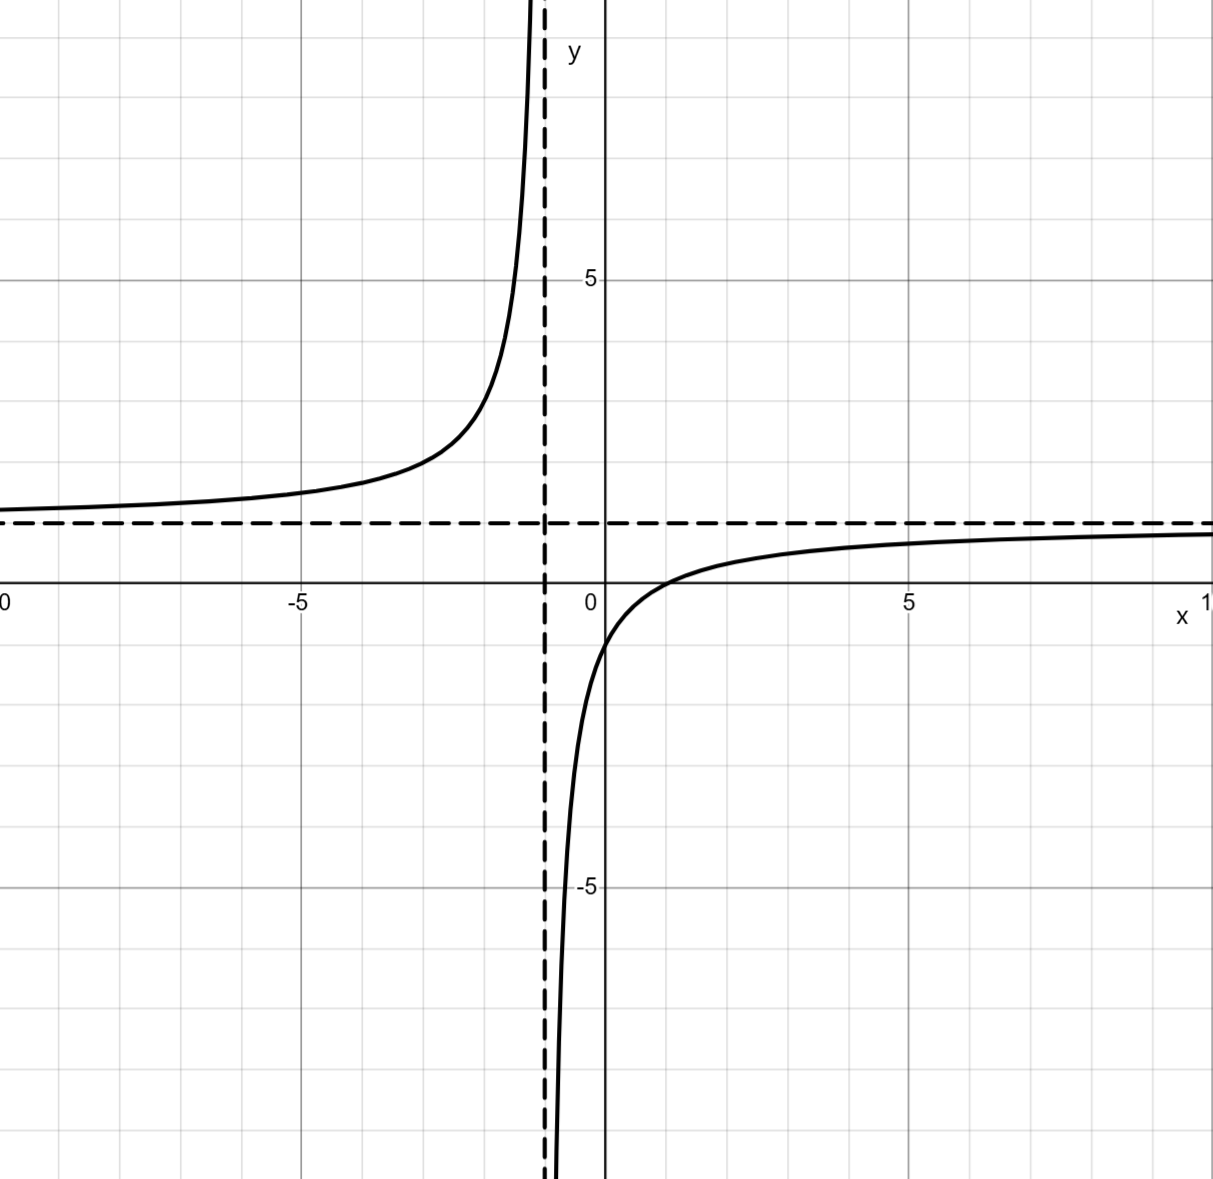
\includegraphics[width=0.5\linewidth]{img/2_lomena_fkce.png}
        \caption{$f(x):$ $y=\frac{x-1}{x+1}$} (čerchovaně jsou asymptoty)
        \label{fig:enter-label}
    \end{figure}

tato konkrétní funkce je v intervalu $\mathbb{R}-\{1\}$, jelikož v $x = -1$ není definována 
\subsubsection{Asymptoty}
Asymptota je taková přímka, jejíž vzdálenost od křivky se limitně blíží k nule, když se jedna nebo obě souřadnice blíží nekonečnu. \\ \\
Co to znamená? funkce se blíží k dané asymptotě do nekonečna, nikdy ji neprotne.\\ \\
Příklad: Určete asymptoty $y=\frac{2x-3}{x-1}$\\
Budou 2 asymptoty. \\
1. získáme určením podmínky $x \neq 1$ první asymptota má rovnici: $x=1$ \\
2. získáme podílem $(2x-3):(x-1)=2\cdot(-\frac{1}{x-1})$. Druhá asymptota má tedy hodnotu $y=2$
graf funkce je:
\begin{figure}[H]
        \centering
        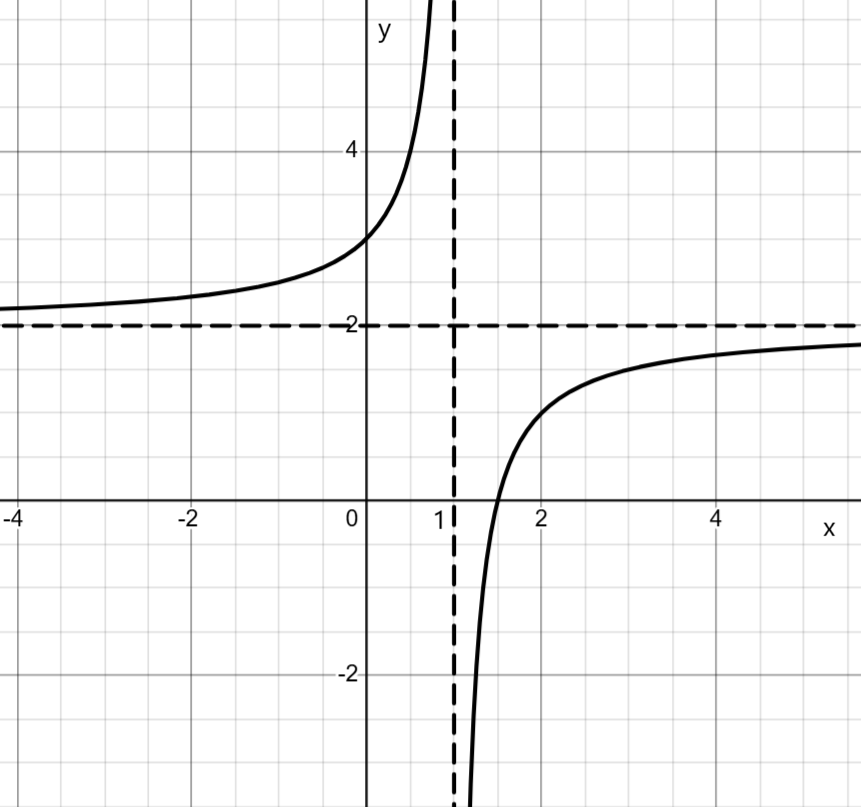
\includegraphics[width=0.5\linewidth]{img/2_lomena_fkce2.0.png}
        \caption{$f(x):$ $y=\frac{2x-3}{x-1}$} (čerchovaně jsou asymptoty)
        \label{fig:enter-label}
    \end{figure}
    

\subsection{Základní vlastnosti funkcí}
\subsubsection{Definiční obor}
Množina $A$ označujeme $D(f)$ a platí pro ni, že $x \in A$
\subsubsection{Obor hodnot}
Obor hodnot je množinou prvků $y \in B$ z nichž ke každému existuje alespoň jeden takový prvek $x\in A$, že $[x,y] \in f$ nazíváme oborem hodnot funkce $f$ a označujeme $H(f)$
\subsubsection{Intervaly monotónnosti}
Intervaly (souvislá množina hodnot), ve kterých je funkce rostoucí nebo klesající
\subsubsection{Sudost Lichost}
Funkce je sudá (souměrná podle osy $y$), pokud splňuje: když do funkce vložíte prvek $x$ a poté inverzní prvek $-x$, pak musí funkce vrátit stejnou výslednou hodnotu. Typickou sudou funkcí je funkce $f: y=x^2$ \\

Funkce se nazývá lichá (je souměrná podle počátku $[0;0]$), pokud splňuje:  \\
1) Pro každé $x \in D(f)$ je také $-x \in D(f)$ \\
2) Pro každé $x \in D(f)$ je $f(-x) = - f(x)$
například funkce: $y=x^3$
\subsubsection{Prostá funkce}
Prostá funkce je v funkcí, která žádnou funkční hodnotu nenabývá vícekrát
\subsection{Grafy vybraných funkcí a jejich vlastnosti}
\subsubsection{Funkce absolutní hodnoty}
\begin{figure}[H]
        \centering
        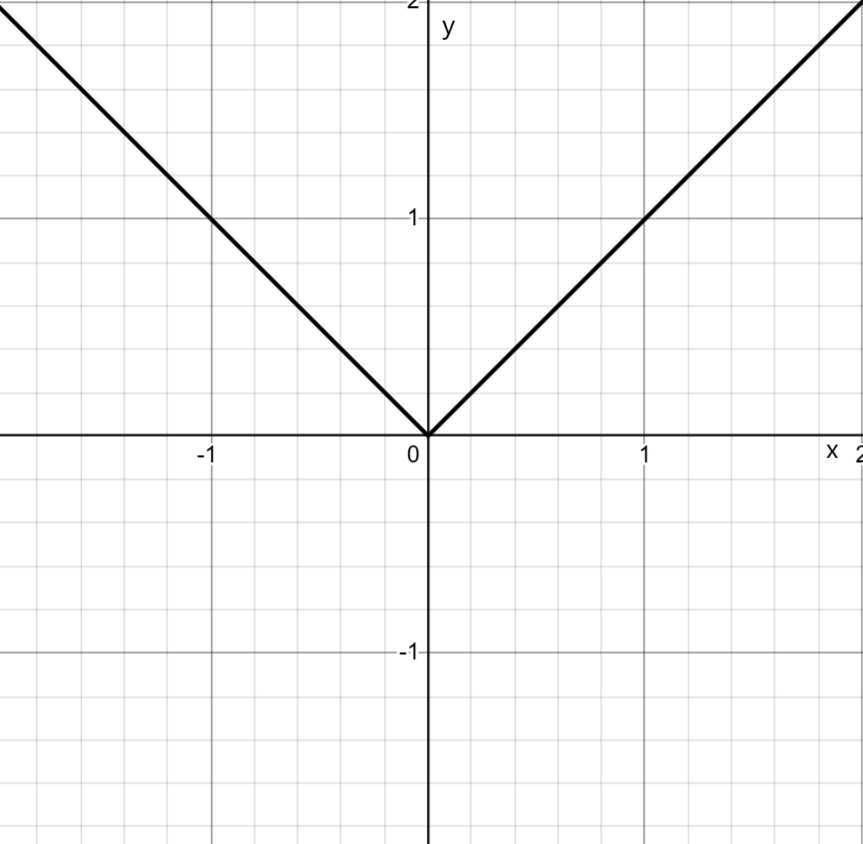
\includegraphics[width=0.5\linewidth]{img/2_absolutni_hodnota.png}
        \caption{$f(x):$ $y=|x|$} 
        \label{fig:enter-label}
    \end{figure}
V intervalu $(-\infty; 0> $ je funkce klesající. V intervalu $<0;\infty)$ je rostoucí. funkce je zdola omezená (má minimum v bodě $[0;0]$). Je sudá.
$$
    D(f)\in \mathbb{R} 
$$
$$
    H(f)\in\langle0;\infty)
$$
\subsubsection{Logaritmická funkce}
\begin{figure}[H]
        \centering
        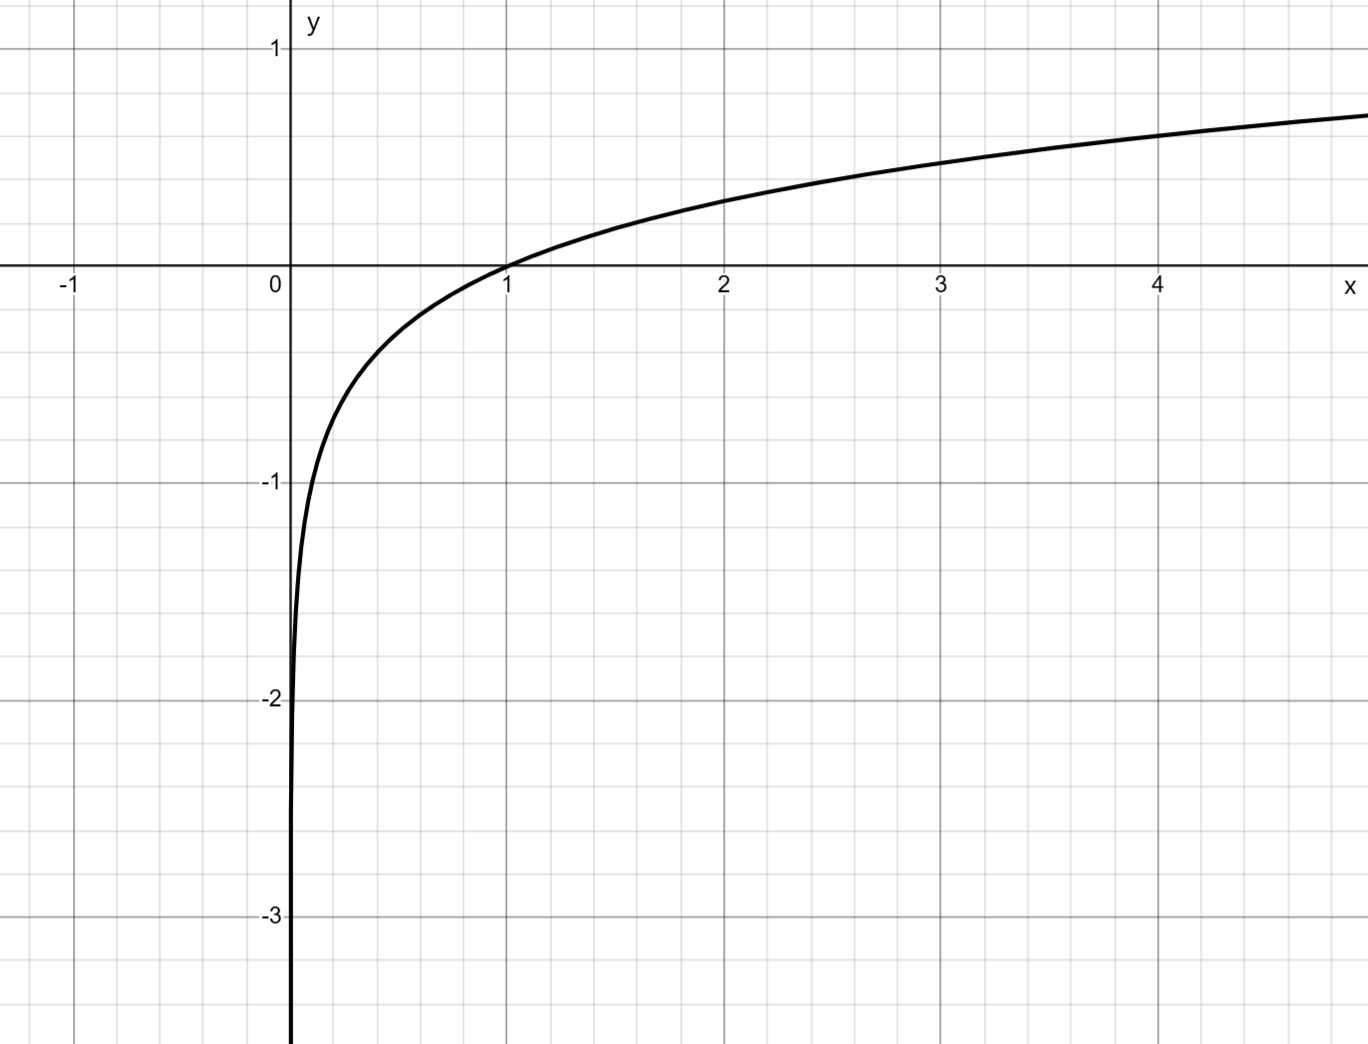
\includegraphics[width=0.5\linewidth]{img/2_logaritmus.png}
        \caption{$f(x): y=log_{10}x$} 
        \label{fig:enter-label}
    \end{figure}
funkce je v celém jejím intervalu $(0;\infty)$ rostoucí. Není omezená. Má lymitu $x=0$
$$
    D(f)\in  (0;\infty)
$$
$$
    H(f)\in\mathbb{R}
$$
\subsubsection{Graf funkce druhé odmocniny}
\begin{figure}[H]
        \centering
        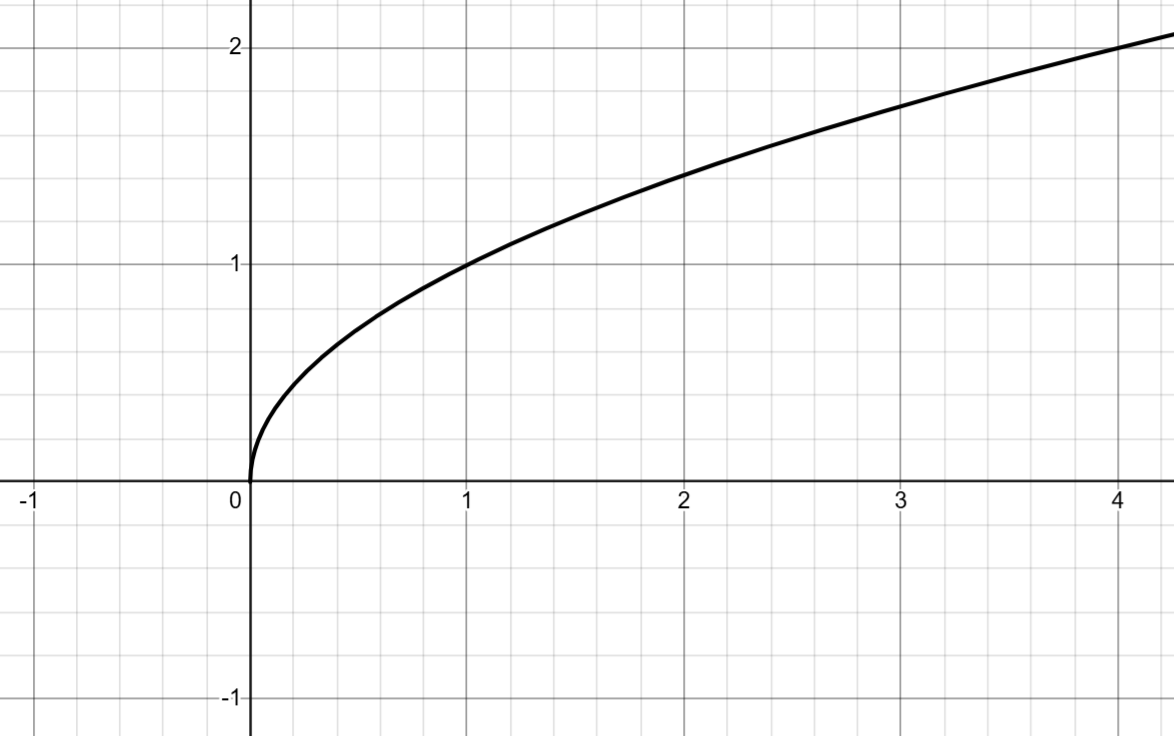
\includegraphics[width=0.5\linewidth]{img/2_odmocnina(x).png}
        \caption{$f(x): y=\sqrt{x}$} 
        \label{fig:enter-label}
    \end{figure}
funkce je v celém jejím intervalu $(0;\infty)$ rostoucí. Je zdola omezená v bodě $[0;0]$
$$
    D(f)\in \langle0;\infty)
$$
$$
    H(f)\in\langle0;\infty)
$$
\subsubsection{Graf funkce třetí odmocniny}
\begin{figure}[H]
        \centering
        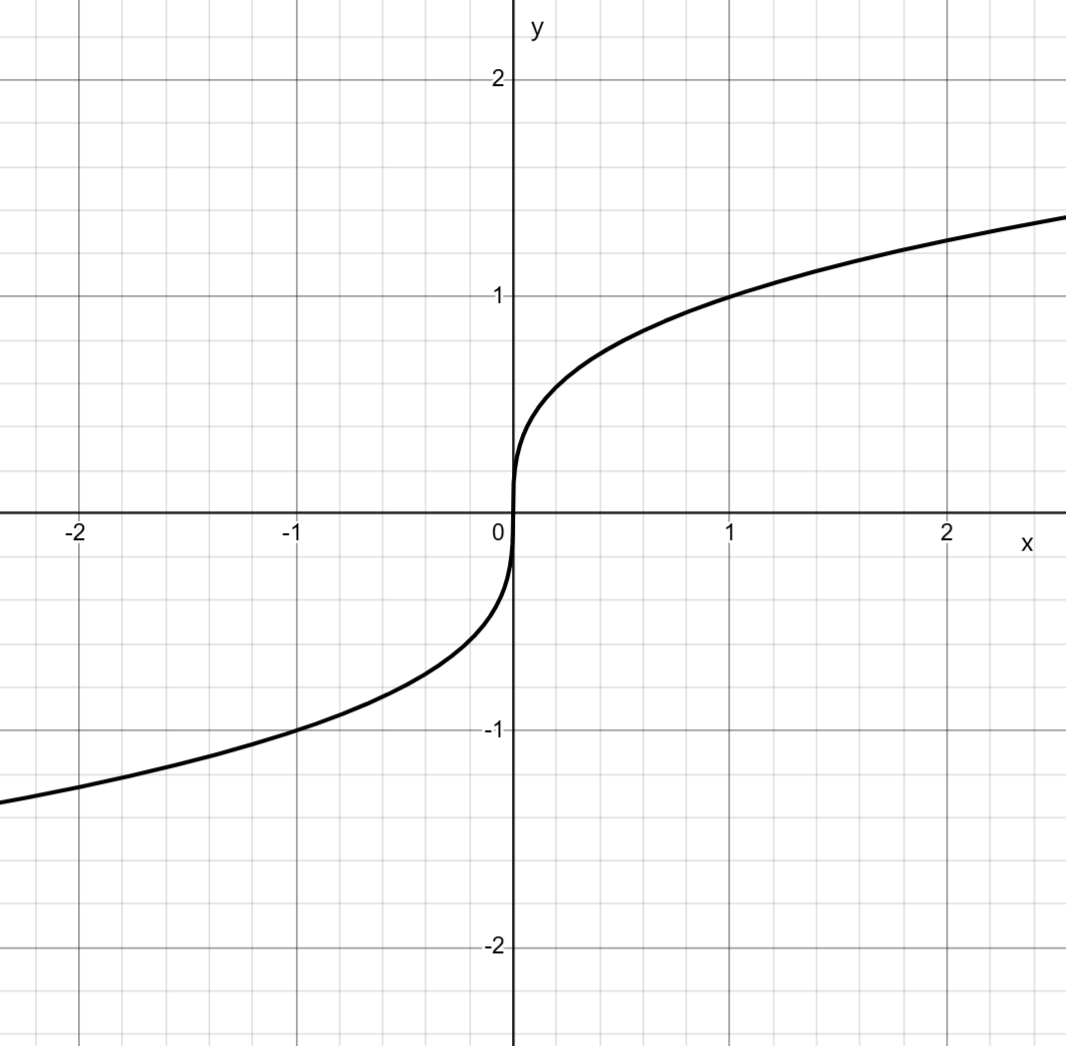
\includegraphics[width=0.5\linewidth]{img/2_3odmocnina(x).png}
        \caption{$f(x): y=\sqrt[3]{x}$} 
        \label{fig:enter-label}
    \end{figure}
funkce je rostoucí
$$
    D(f)\in \mathbb{R} 
$$
$$
    H(f)\in \mathbb{R}
$$



